%%%%%%%%%%%%%%%%%%%%%%%%%%%%%%%%%%%%%%%
% Deedy - One Page Two Column Resume
% LaTeX Template
% Version 1.2 (16/9/2014)
%
% Original author:
% Arighna Chakraborty (https://arighna-chakraborty.netlify.app)
%
% Original repository:
% https://github.com/riju-stone/dev-cv
%
% IMPORTANT: THIS TEMPLATE NEEDS TO BE COMPILED WITH XeLaTeX
%
% This template uses several fonts not included with Windows/Linux by
% default. If you get compilation errors saying a font is missing, find the line
% on which the font is used and either change it to a font included with your
% operating system or comment the line out to use the default font.
% 
%%%%%%%%%%%%%%%%%%%%%%%%%%%%%%%%%%%%%%


\documentclass[]{dev-cv}
\usepackage{fancyhdr}
\usepackage{graphicx}
 
\pagestyle{fancy}
\fancyhf{}
 
\begin{document}

%%%%%%%%%%%%%%%%%%%%%%%%%%%%%%%%%%%%%%
%
%     TITLE NAME
%
%%%%%%%%%%%%%%%%%%%%%%%%%%%%%%%%%%%%%%
\namesection{Arighna}{Chakraborty}{\urlstyle{same}
+91 9163411820 \textbf{|}   
\href{mailto:riju23chakra@gmail.com}{riju23chakra@gmail.com}
}

%%%%%%%%%%%%%%%%%%%%%%%%%%%%%%%%%%%%%%
%
%     COLUMN ONE
%
%%%%%%%%%%%%%%%%%%%%%%%%%%%%%%%%%%%%%%

\begin{minipage}[t]{0.33\textwidth} 


%%%%%%%%%%%%%%%%%%%%%%%%%%%%%%%%%%%%%%
%     PICTURE(OPTIONAL)
%%%%%%%%%%%%%%%%%%%%%%%%%%%%%%%%%%%%%%
\vspace{\topsep}
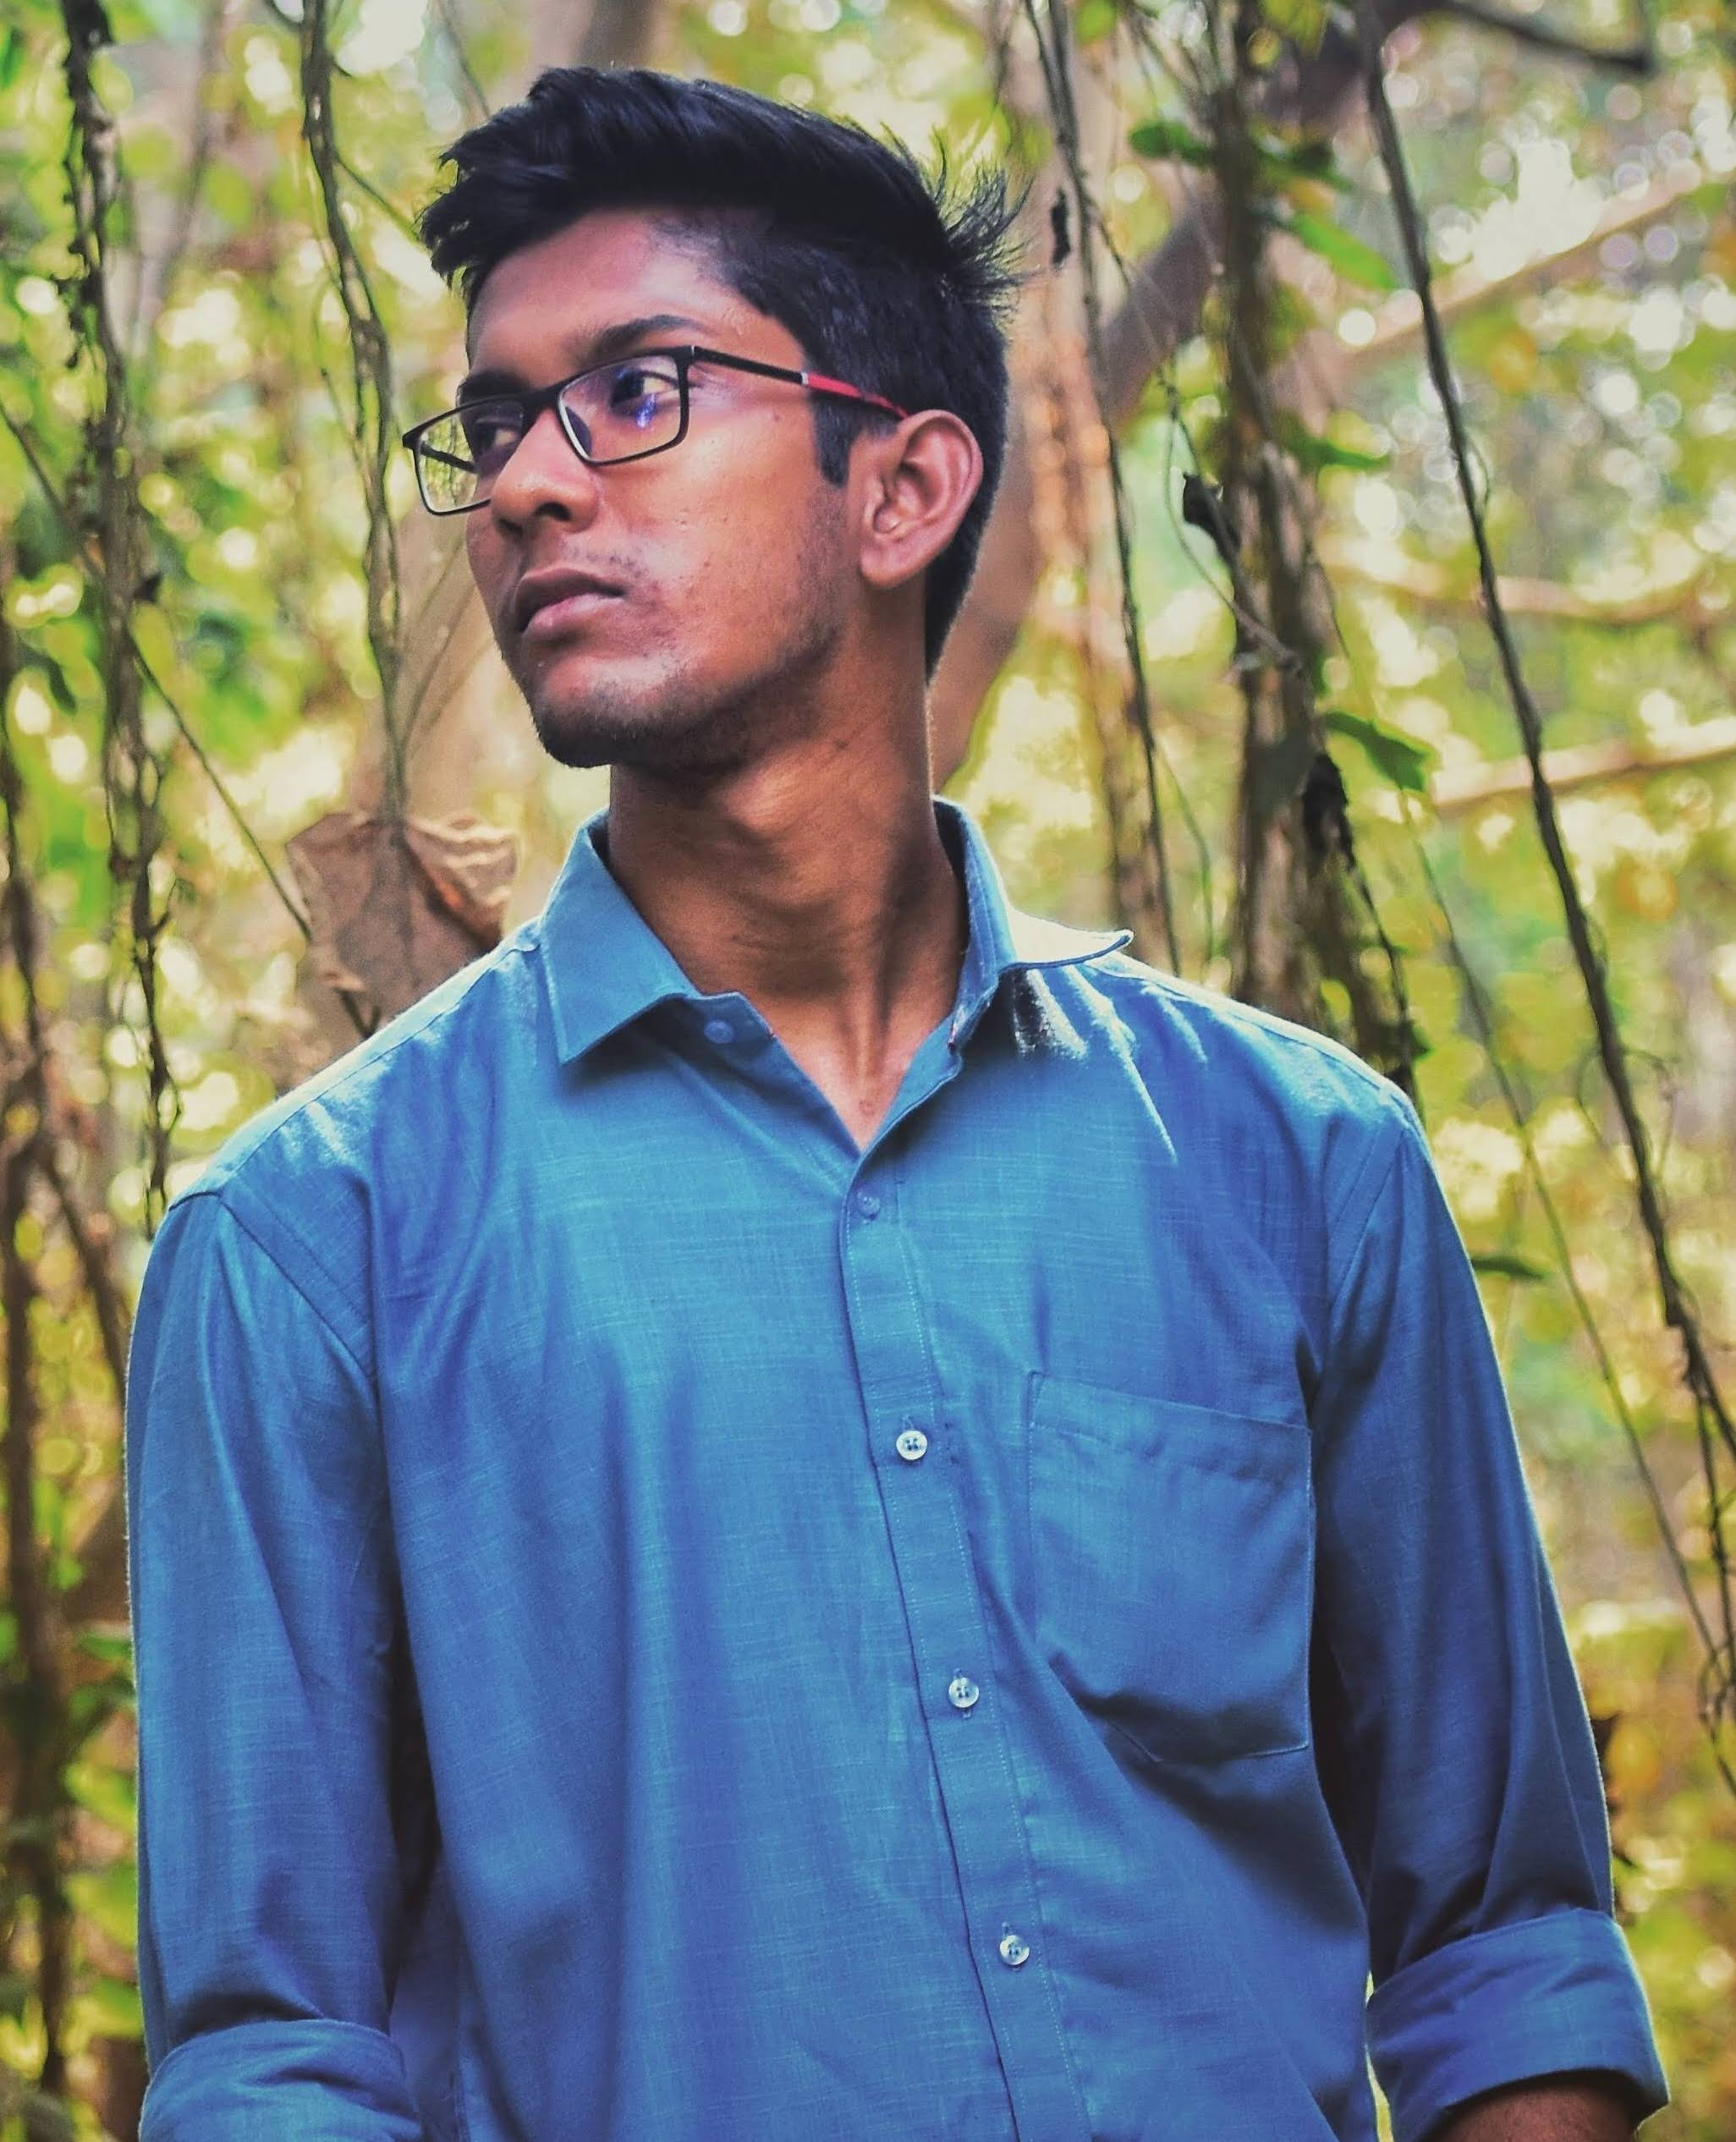
\includegraphics[width=0.65\textwidth]{riju.jpeg}
\sectionsep

%%%%%%%%%%%%%%%%%%%%%%%%%%%%%%%%%%%%%%
%     LINKS
%%%%%%%%%%%%%%%%%%%%%%%%%%%%%%%%%%%%%%

\section{Links} 
Github: \href{https://github.com/riju-stone}{\bf riju-stone} \\
LinkedIn: \href{https://www.linkedin.com/in/arighna-chakraborty-509539113/}{\bf arighna-chakraborty} \\
Twitter: \href{https://twitter.com/RijuStone}{\bf @RijuStone} \\
\sectionsep

%%%%%%%%%%%%%%%%%%%%%%%%%%%%%%%%%%%%%%
%     EDUCATION
%%%%%%%%%%%%%%%%%%%%%%%%%%%%%%%%%%%%%%

\section{Education}

\runsubsection{St. Xaviers College} \\
\descript{M.Sc. in Computer Science}
\location{Jun 2022 | Kolkata, India}
\sectionsep

\runsubsection{Vidyasagar College}  \\
\descript{B.Sc. in Computer Science}
\location{Sept 2020 | Kolkata, India}
\sectionsep

\runsubsection{Pearls of God School}    \\
\location{May 2017 |  Hooghly, India}
\sectionsep

%%%%%%%%%%%%%%%%%%%%%%%%%%%%%%%%%%%%%%
%     SKILLS
%%%%%%%%%%%%%%%%%%%%%%%%%%%%%%%%%%%%%%

\section{Skills}
\subsection{Programming}
\location{Over 5000 lines:}
JavaScript \textbullet{} Java \\
CSS \textbullet{} HTML  \\
\vspace{\topsep}
\location{Over 1000 lines:}
C++ \textbullet{} Python \\
\vspace{\topsep}
\location{Familiar:}
SQL \textbullet{} Go \textbullet{} Prolog
\vspace{\topsep}
\subsection{Frameworks}
Flutter \textbullet{} React \textbullet{} Electron \\
\sectionsep

%%%%%%%%%%%%%%%%%%%%%%%%%%%%%%%%%%%%%%
%   HOBBIES (IF ANYTHING APPROPRIATE)
%%%%%%%%%%%%%%%%%%%%%%%%%%%%%%%%%%%%%%

%%%%%%%%%%%%%%%%%%%%%%%%%%%%%%%%%%%%%%
%
%     COLUMN TWO
%
%%%%%%%%%%%%%%%%%%%%%%%%%%%%%%%%%%%%%%

\end{minipage} 
\hfill
\begin{minipage}[t]{0.66\textwidth} 

%%%%%%%%%%%%%%%%%%%%%%%%%%%%%%%%%%%%%%
%     ABOUT
%%%%%%%%%%%%%%%%%%%%%%%%%%%%%%%%%%%%%%
\section{About}
\descript{Web Developer | App Developer}
\vspace{\topsep}
Aspiring developer with hands-on experience in latest web and app development frameworks such as React and Flutter. Highly organised and detail-oriented with focus on learning and developing open-source projects to further strengthen my knowledge.
\sectionsep

%%%%%%%%%%%%%%%%%%%%%%%%%%%%%%%%%%%%%%
%     EXPERIENCE
%%%%%%%%%%%%%%%%%%%%%%%%%%%%%%%%%%%%%%
\section{Experience}
% \runsubsection{ Simulacra Technologies }
% \descript{| Web Developer Intern }
% \location{Nov 2021 - Present | Kolkata, IN}
% \vspace{\topsep}
% \vspace{\topsep}
% \begin{tightemize}
% \item Worked on numerous frontend projects using React and Tailwindcss frameworks
% \item Worked on simple backend systems and Restful APIs using Go.
% \end{tightemize}
% \sectionsep

\runsubsection{ \href{https://www.skillacademia.in/}{Skill Academia} }
\descript{|  Software Developer Intern }
\location{May 2021 – Oct 2021 | Kolkata, IN}
\vspace{\topsep}
\begin{tightemize}
\item App Development - developed a cross-platform mobile application built with Flutter and Firebase 
\item Frontend Development - Wrote and reviewed code for company website using ReactJs
\end{tightemize}
\sectionsep

%%%%%%%%%%%%%%%%%%%%%%%%%%%%%%%%%%%%%%
%     PROJECTS
%%%%%%%%%%%%%%%%%%%%%%%%%%%%%%%%%%%%%%

\section{Projects}
\runsubsection{\href{https://github.com/riju-stone/chatbot}{Chatbot}} \\
\location{2021}
\vspace{\topsep}
This project is a part of our final year post-graduate curriculum. A team of three students including me, are currently working on a Hybrid Chatbot which possesses both Retrieval and Generative response generation modules.  
\sectionsep

\runsubsection{\href{https://github.com/riju-stone/dictator}{Dictator}} \\
\location{2021}
\vspace{\topsep}
A voice note app that listens to your mic or speaker and takes down everything it hears. Built using ReactJs and Electron framework.
\sectionsep 

\runsubsection{\href{https://github.com/riju-stone/covid-track}{Covid Track}}\\
\location{2020}
\vspace{\topsep}
A cross-platform mobile application made with Flutter and Firebase to track and provide latest COVID stats and news.
\sectionsep

\runsubsection{\href{https://github.com/riju-stone/chess}{Chess}}  \\
\location{2019}
\vspace{\topsep}
Created a simple cross-platform desktop application for a Chess GUI using Electron framework.
\sectionsep

%%%%%%%%%%%%%%%%%%%%%%%%%%%%%%%%
%   Publications
%%%%%%%%%%%%%%%%%%%%%%%%%%%%%%%%

\end{minipage} 
\end{document}  \documentclass[]{article}
